%%%%%%%%%%%%%%%%%%%%%%% file template.tex %%%%%%%%%%%%%%%%%%%%%%%%%
%
% This is a general template file for the LaTeX package SVJour3
% for Springer journals.          Springer Heidelberg 2010/09/16
%
% Copy it to a new file with a new name and use it as the basis
% for your article. Delete % signs as needed.
%
% This template includes a few options for different layouts and
% content for various journals. Please consult a previous issue of
% your journal as needed.
%
%%%%%%%%%%%%%%%%%%%%%%%%%%%%%%%%%%%%%%%%%%%%%%%%%%%%%%%%%%%%%%%%%%%
%
% First comes an example EPS file -- just ignore it and
% proceed on the \documentclass line
% your LaTeX will extract the file if required
\begin{filecontents*}{example.eps}
    %!PS-Adobe-3.0 EPSF-3.0
    %%BoundingBox: 19 19 221 221
    %%CreationDate: Mon Sep 29 1997
    %%Creator: programmed by hand (JK)
    %%EndComments
    gsave
    newpath
    20 20 moveto
    20 220 lineto
    220 220 lineto
    220 20 lineto
    closepath
    2 setlinewidth
    gsave
    .4 setgray fill
    grestore
    stroke
    grestore
\end{filecontents*}
%
\RequirePackage{fix-cm}
%
\documentclass{svjour3}                     % onecolumn (standard format)
%\documentclass[smallcondensed]{svjour3}     % onecolumn (ditto)
%\documentclass[smallextended]{svjour3}       % onecolumn (second format)
%\documentclass[twocolumn]{svjour3}          % twocolumn
%
\smartqed  % flush right qed marks, e.g. at end of proof
%
\usepackage{graphicx}
%
% \usepackage{mathptmx}      % use Times fonts if available on your TeX system
%
% insert here the call for the packages your document requires
%\usepackage{latexsym}
% etc.
%
% please place your own definitions here and don't use \def but
% \newcommand{}{}
%
% Insert the name of "your journal" with
% \journalname{myjournal}
%
\begin{document}

    \title{Neural Networks and their Application in Reinforcement Learning%\thanks{Grants or other notes
    %about the article that should go on the front page should be
    %placed here. General acknowledgments should be placed at the end of the article.}
    }
    \subtitle{Reinforcement Learning Seminar -- Winter Semester 2018/19}

    %\titlerunning{Short form of title}        % if too long for running head

    \author{Fabian Otto
    %    \and Second Author %etc.
    }

    %\authorrunning{Short form of author list} % if too long for running head

    \institute{Fabian Otto \at
    Technische Universit\"at Darmstadt, Computer Science Department\\
    %    Tel.: +123-45-678910\\
    %    Fax: +123-45-678910\\
    \email{fabian.otto@stud.tu-darmstadt.de}           %  \\
    %             \emph{Present address:} of F. Author  %  if needed
    %    \and
    %    S. Author \at
    %    second address
    }

    \date{Received: date / Accepted: date}
    % The correct dates will be entered by the editor


    \maketitle

    \begin{abstract}
        Insert your abstract here. Include keywords, PACS and mathematical
        subject classification numbers as needed.
        \keywords{Reinforcement Learning\and Neural Networks}
        % \PACS{PACS code1 \and PACS code2 \and more}
        % \subclass{MSC code1 \and MSC code2 \and more}
    \end{abstract}

    \section{Introduction}
    \label{sec:intro}
    Give introduction with NN hype or similar things. As well as the importance.
    Define RL and the method in general.
    Show clear distinction to SL.
    Maybe include success of recent things in CV and NLP, might also be possible in \ref{sec:history} to transition to more recent approaches in RL. 
    Introduce RL goal and notation, short intro ro MDPs.
    \section{Definition of Neural Networks}
    \label{sec:def}
    \cite{RefB} and \cite{RefJ}.
    Describe formally how NN are working, how can they be trained, what other methods do we have, etc.
    \section{History of Neural Networks}
    \label{sec:history}
    (see Sect.~\ref{sec:1}).
    What did lead to the rise and fall of NNs throughout time.
    Create good transition to recent approaches.


%    \section{Recent Approaches in Reinforcement Learning}
%    \label{sec:recent}
    \section{Algorithms}
	    \label{sec:algo}
	    This section provides an overview of NN based RL algorithms including earlier work and its improvements as well as current state-of-the-art. 
	    Most algorithms can be either classified as on-policy or off-policy algorithms.
		On-policy algorithms estimate the value of policy while using it for control whereas in off-policy algorithms, the generating policy, called \textit{behavior policy}, is not necessarily related to the \textit{target policy}, which is improved and evaluated.
		This allows to use a deterministic target policy, while sampling all actions applying the behavior policy. \cite[chapter 5]{Sutton2018}
		
 	\subsection{Off-Policy}
 	\paragraph{MDPs}
		\label{sec:off-policy}
		One of the earlier NN based off-policy algorithms, named Neural fitted Q Iteration (NFQ), was published by Riedmiller \cite{Riedmiller2005} in 2005. 
		NFQ is a model-free algorithm, based on Q-Learning \cite{Watkins1989} and approximates the action-value function with multilayer-perceptrons.
		Compared to other approaches at the time, NFQ allows to learn with a relatively good data efficiency.
		Further, batches from a replay memory \cite{Lin1992} are used in order to train the multilayer-perceptron with resilient backpropagation (RPROP) \cite{Riedmiller1993}.
		Thereby, it is possible to dynamically add new samples to the replay memory during learning.
		Motivated by this idea as well as the success of TD-gammon \cite{Tesauro1994} the arguably biggest improvement in NN based RL -- Deep Q-Networks (DQN) -- were introduced by Mnih, et al. \cite{Mnih2015}.   
		They built upon their prior results \cite{Mnih2013} on the Atari Arcade Environment \cite{Bellemare2013} which already achieved state-of-the-art performance for some of the games.
		DQNs introduce better scalability to larger data sets by replacing NFQ's RPROP with Stochastic Gradient Descent (SGD) updates. 
		Further, they allow training end-to-end from the raw visual input utilizing convolutional neural networks. 
		Benchmarks of more recent version \cite{Mnih2015} show an improved performance as well as a better generalization to more Atari games compared to initial work \cite{Mnih2013}.
		The performance improvement was mainly achieved by introducing a second target Q-network, which is only periodically updated and thereby reduces sample correlations. 
		However, van Hasselt, et al. \cite{VanHasselt2016} show that the current DQN \cite{Mnih2015} approach is not sufficient to avoid overestimations of action-values under certain conditions. 
		This in itself is not harmful to the policy's performance, but if the overestimation is not uniform and not concentrated at the states of interest, it might affect the policy negatively. 
		To mitigate the risk of overestimation, they propose Double DQN (DDQN).
		Double Q-Learning in general tries to decouple the selection and evaluation of actions by learning two action-value functions. 
		One determines the greedy policy and the other the value of this policy.  
		In order to reduce the computational cost, van Hasselt, et al. utilize the already existing online Q-network for determining the greedy policy and the target Q-network for estimating its value. 
		Further, this allows them to achieve better performance on most of the Atari games. 
		Decoupling is also done in a more extreme form with Dueling Double DQNs (DDDQN) from Wang, et al. \cite{Wang2016}. 
		They introduce two separate function approximators, one for the state-value function and one for the state dependent action advantage function, in order to represent the action-value\footnote{Both estimators share parameters in the networks's convolutional part and are trained together end-to-end.}.
		These approximators allow the dueling architecture to learn about the value of a state regardless of the action taken. 
		This is especially important as in many states, the action has no repercussions about the near future. 
		Additional improvements, include gradient clipping and prioritized experience replay (PER) \cite{Schaul2015}.
		Combining PER with DDQN \cite{Schaul2015} showed that sampling rare experiences with a higher probability makes learning with replay memories more efficient \cite{Lin1992}. 
		However, sampling non-uniformly from the replay memory introduces a bias, that has to be corrected during the update step.\\
		All previous approaches are using environments, which do not have to deal with delayed and sparse feedback.
		In real world applications this is often not the case and algorithms still need the ability to learn.
		One key problem, which arises during training, is insufficient exploration, thereby unstable policies. 
		Using intrinsically motivated agents, exploration can be achieved for the agent itself rather for an external goal. 
		This idea is implemented by Kulkarni, et al. \cite{Kulkarni2016} in hierarchical-DQN (h-DQN), which is based on a hierarchy of two DQNs.
		A top level \textit{meta-controller} is selecting a subgoal in order to optimize the extrinsic reward.
		The lower level \textit{controller} maximizes an intrinsic reward by solving the subgoal.
		This allows h-DQN to achieve a significant better performance on the Atari game Montezuma's Revenge.\\
		As the above results show, classical Q-learning \cite{Watkins1989} is quite successful for discrete action spaces, real world problems however often require continuous action spaces.
		Lillicrap, et al. \cite{Lillicrap2016} adapt the idea of DQN \cite{Mnih2015} and make it applicable to the continuous action domain. 
		They introduce Deep Deterministic Policy Gradients (DDPG), a model-free Actor-Critic (AC) algorithm with approximate Q-Learning based on deterministic policy gradients (DPG) \cite{Silver2014}.
		DQN's \cite{Mnih2015} architecture is improved by adding batch normalization layers \cite{Ioffe2015} to deal with different physical units in the observation space. 
		In order to stabilize policies, they adapt the idea of target networks from DQN \cite{Mnih2015} and use "soft" target updates for AC. 
		Besides continuous action spaces, it is usually hard to collect data from e.g. robots, and therefore dealing with high sample complexity in real world applications.
		Normalized advantage functions (NAF) \cite{Gu2016} approaches this problem with a DQN based algorithm.
		Similar to DDDQN \cite{Wang2016}, the Q-network is represented by one state-value function output and one state dependent action advantage function.
		In order to reduce sample complexity, NAF incorporates \textit{imagination rollouts}. 
		Those synthetic on-policy samples are created by utilizing a mixture of iterative LQG (iLQG) \cite{Todorov2005} and on-policy trajectories for real world rollouts.
		Afterwards, the learned model for the states is used to generate replay memory entries. 
		This can be seen as a scalable variant of Dyna-Q \cite{Sutton1990}. 
		As a drawback, NAF failed to show improvements using iLQG compared to on-policy samples, however, iLQG might be desirable when avoiding damaging actions is critical. 
		
		
%		In order to reduce sample complexity they do not require a second actor or policy. 
		
		
 	\paragraph{POMDPs}
    \subsection{On-Policy}
    \label{sec:on-policy}
	
    \subsection{Real World Applications}
    \label{sec:games}
    Talk about DeepMinds AlphaZero, TDGammon, Atari Game Systems, e.g. Minh
    But also applications outside of Games, maybe seperate this into two different subsections.
    \paragraph{Paragraph headings}
    % For one-column wide figures use
    \begin{figure}
        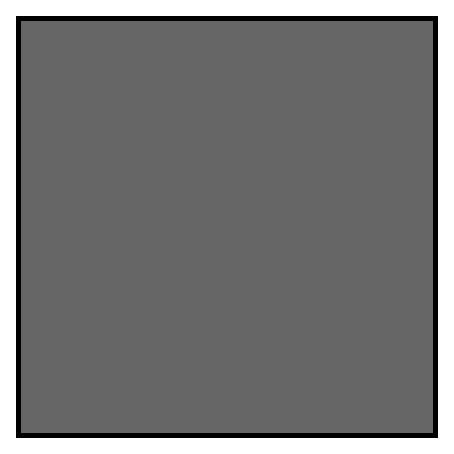
\includegraphics{example.eps}
        % figure caption is below the figure
        \caption{Please write your figure caption here}
        \label{fig:1}
    \end{figure}
    %
    % For two-column wide figures use
    \begin{figure*}
        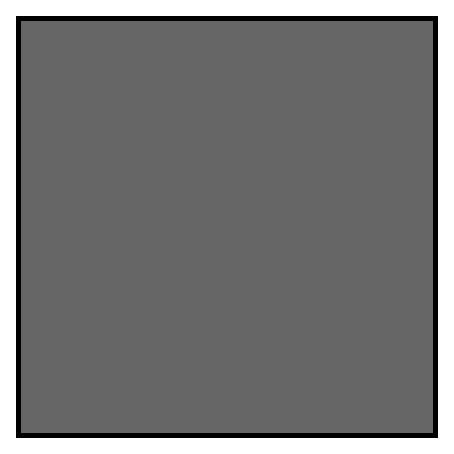
\includegraphics[width=0.75\textwidth]{example.eps}
        % figure caption is below the figure
        \caption{Please write your figure caption here}
        \label{fig:2}
    \end{figure*}

    \begin{table}
        % table caption is above the table
        \caption{Please write your table caption here}
        \label{tab:1}
        \begin{tabular}{lll}
            \hline\noalign{\smallskip}
            first & second & third  \\
            \noalign{\smallskip}\hline\noalign{\smallskip}
            number & number & number \\
            number & number & number \\
            \noalign{\smallskip}\hline
        \end{tabular}
    \end{table}


    %\begin{acknowledgements}
    %If you'd like to thank anyone, place your comments here
    %and remove the percent signs.
    %\end{acknowledgements}

    % BibTeX users please use one of
    %\bibliographystyle{spbasic}      % basic style, author-year citations
    \bibliographystyle{spmpsci}      % mathematics and physical sciences
    %\bibliographystyle{spphys}       % APS-like style for physics
    \bibliography{library.bib}
    % name your BibTeX data base

\end{document}

